%% mitl_paper.tex
%% Manual-in-the-Loop (MITL): Specification-Derived Constraint Projection
%% for ICS Anomaly Detection
%%
%% Target: AISec @ CCS 2027 (or CRITIS 2026)
%% Format: ACM CCS (acmart, sigconf)
%% Author: sassom2112 <sassom2112@gmail.com>
%%
%% TODO markers flag results pending HAI 22.04 real-data runs (Sprint 9 on Kaggle)
%% and the Bedrock LLM extraction ablation (Sprint 11).
%%
\documentclass[sigconf,anonymous,review]{acmart}

\usepackage{booktabs}
\usepackage{listings}
\usepackage{microtype}
\usepackage{xcolor}
\usepackage{tikz}
\usetikzlibrary{arrows.meta, positioning, shapes.geometric, fit, backgrounds}
\usepackage{amsmath}

%% -- Metadata ----------------------------------------------------------------
\acmConference[AISec '27]{ACM Workshop on Artificial Intelligence and Security}{%
  November 2027}{Salt Lake City, UT, USA}
\acmDOI{}
\acmISBN{}

\newcommand{\mitl}{\textsc{mitl}\xspace}
\newcommand{\catt}{\textsc{catt}\xspace}
\newcommand{\todo}[1]{\textcolor{red}{[TODO: #1]}}

% ─────────────────────────────────────────────────────────────────────────────
\begin{document}

\title{Manual-in-the-Loop (MITL): Specification-Derived Constraint Projection
       for ICS Anomaly Detection}

\author{Anonymous Author(s)}
\affiliation{\institution{Anonymous Institution}}
\email{anonymous@institution.edu}

\begin{abstract}
Statistical machine learning applied to industrial control system (ICS) network
traffic plateaus at 49.9\% recall on replay attacks — because replay uses
valid protocol packets that are statistically indistinguishable from normal
traffic.  We introduce \emph{Manual-in-the-Loop} (\mitl): a
specification-derived constraint layer that encodes physical system invariants
directly from engineering documentation, without requiring any labeled attack
data.  \mitl detects attacks by enforcing cross-layer structural invariants
that no density model can observe — specifically, the physical impossibility of
elevated Modbus command traffic co-occurring with frozen valve actuator states.

On the ICSSim v2 water-treatment simulator, \mitl-Static (spec-only, no
calibration) achieves 25\% replay recall at zero observational cost, while
\mitl-Calibrated (spec $+$ 15\% unlabeled warm-up) achieves 100\% replay
recall — both with zero attack labels.  On the HAI 22.04 steam-turbine
benchmark evaluated with eTaPR, \mitl detects AP27-class sensor spoofing that
statistical baselines miss entirely~\todo{fill after Sprint 9 Kaggle run}.
We release \mitl as an open-source pip-installable library with reference
encodings for both datasets and an AWS Bedrock LLM extraction backend that
generalises the framework to any ICS engineering manual.

\mitl is the detection-side companion to \catt~\cite{catt2026}, which showed
that the same constraint projection mechanism exposes inflated evasion rates
in adversarial NIDS evaluation.  The constraint layer is the unifying
abstraction: \catt uses it to bound attack perturbations; \mitl uses it to
define what normal physical operation cannot violate.
\end{abstract}

\begin{CCSXML}
<ccs2012>
  <concept>
    <concept_id>10002978.10003006.10003007</concept_id>
    <concept_desc>Security and privacy~Intrusion detection systems</concept_desc>
    <concept_significance>500</concept_significance>
  </concept>
  <concept>
    <concept_id>10010147.10010257</concept_id>
    <concept_desc>Computing methodologies~Machine learning</concept_desc>
    <concept_significance>300</concept_significance>
  </concept>
</ccs2012>
\end{CCSXML}

\ccsdesc[500]{Security and privacy~Intrusion detection systems}
\ccsdesc[300]{Computing methodologies~Machine learning}

\keywords{ICS security, OT anomaly detection, constraint projection,
          specification-based detection, replay attacks, MITL, eTaPR}

\maketitle

% ─────────────────────────────────────────────────────────────────────────────
\section{Introduction}
\label{sec:intro}

Operational technology (OT) networks differ from enterprise networks in a way
that undermines standard ML-based intrusion detection: attacks do not have to
look anomalous at the network layer.  A \emph{replay attack} captures
legitimate Modbus control traffic and re-transmits it verbatim.  Every
individual packet is valid; the statistical distribution of protocol fields
is normal.  An ML classifier trained on network features cannot distinguish
replay traffic from normal traffic by design — the attacker copied it.

The consequences are physical.  In the ICSSim v2 water-treatment simulator,
a replay attack freezes the input valve actuator register at a captured
position while the real process continues.  The physical system diverges from
the controller's model of it.  A tank that should be draining does not drain;
a tank that should be filling overflows.  The network classifier sees nothing
wrong.  Our best supervised model (LightGBM on 48 network features) achieves
49.9\% replay recall — effectively random~\cite{sprints2026}.

This paper addresses a question that follows directly from this ceiling:
\emph{if you cannot add signal intelligence, what can you add?}  Our answer
is: \textbf{add a manual in the loop}.

Every ICS deployment comes with engineering documentation that specifies
exactly what the physical system must do.  A pressure control loop has
saturation limits.  A speed controller ramps through a specified rate limiter.
A turbine speed sensor must track its setpoint.  These are not statistical
properties — they are structural invariants derivable from the documentation
without observing a single attack.

\mitl encodes these invariants as a constraint layer, calibrates them
against unlabeled warm-up data, and flags any time window where physical
reality violates what the spec says must be true.  The key finding is a
three-tier gradient:
\begin{enumerate}
  \item \textbf{Supervised network ML}: 49.9\% replay recall — structural ceiling.
  \item \textbf{\mitl-Static} (spec-only constraints): 25\% recall — non-zero
        at zero annotation cost.
  \item \textbf{\mitl-Calibrated} (spec $+$ warm-up baseline): 100\% recall —
        full detection without a single attack label.
\end{enumerate}

The gradient is the story.  Not that static thresholds alone are sufficient,
but that the specification encodes \emph{what invariant breaks} during a
replay attack, and warm-up calibration encodes \emph{what normal looks like}.
Neither alone is sufficient; together they close the 49\% ceiling entirely.

\paragraph{Companion to \catt.}
\catt~\cite{catt2026} showed that enforcing a \texttt{ConstraintSpec}
projection layer reveals that adversarial NIDS evasion rates are inflated by
up to 56.8 percentage points when attacks violate domain constraints (negative
packet counts, ports $>$ 65535).  \mitl is the detection-side dual: the same
constraint mechanism, applied not to bound attacker perturbations but to
define what the physical process cannot do during an attack.

\paragraph{Contributions.}
\begin{itemize}
  \item A formal four-constraint MITL framework with typed data contracts and
        spec provenance (page number, figure, verbatim quote).
  \item A three-tier empirical finding on ICSSim v2 demonstrating the
        complementary roles of static spec constraints and warm-up calibration.
  \item eTaPR-based evaluation on the HAI 22.04 benchmark, the harder
        steam-turbine dataset with 58 multi-process attacks.
  \item An open-source pip-installable library (\texttt{pip install mitl})
        with reference encodings for both datasets and an LLM extraction
        backend (AWS Bedrock) for generalisation to new manuals.
\end{itemize}

% ─────────────────────────────────────────────────────────────────────────────
\section{Background}
\label{sec:background}

\subsection{ICS Anomaly Detection}
ICS anomaly detection spans three layers: network (protocol fields, flow
volume), process (sensor readings, PLC state), and specification
(physical invariants from system documentation).  ML-based approaches focus
on layers one and two~\cite{Goh2017,Aoudi2018,Ahmed2018}.  Specification-based
approaches~\cite{Adepu2018,Feng2019} encode domain knowledge as rules but
require expert manual authoring and do not generalise across datasets.
\mitl occupies a third position: it automates the spec-authoring pipeline
via LLM extraction and separates what-is-invariant (spec) from what-is-normal
(warm-up calibration).

\subsection{Replay Attacks in ICS}
Replay attacks capture legitimate Modbus/DNP3 traffic and retransmit it to
deceive controllers~\cite{Mo2009}.  The ICSSim v2 replay implementation
captures a fill/drain command sequence and replays it continuously.  The
replayed commands freeze the input valve register at the captured position
($\texttt{tank\_input\_valve\_status} = $ const).  Network volume increases
because replayed traffic overlays normal polling traffic.  The resulting
cross-layer contradiction — elevated network commands co-occurring with frozen
valve state — is physically impossible under normal operation and is the
signal \mitl encodes as constraint C4.

\subsection{eTaPR Metric}
The HAI dataset mandates eTaPR (Enhanced Time-series Aware Precision and
Recall)~\cite{Hwang2021} rather than point-wise F1.  Point F1 overcounts
recall when a detector fires across an entire attack duration as one long
blob, and penalises early-warning detectors that fire slightly before an
event.  eTaPR scores at the \emph{event} level with a configurable lead-time
buffer (we use $\delta = 60$ seconds): an event is detected if any predicted
segment overlaps $[\text{event\_start} - \delta, \text{event\_end}]$.

% ─────────────────────────────────────────────────────────────────────────────
\section{The MITL Framework}
\label{sec:framework}

\begin{figure*}[t]
\centering
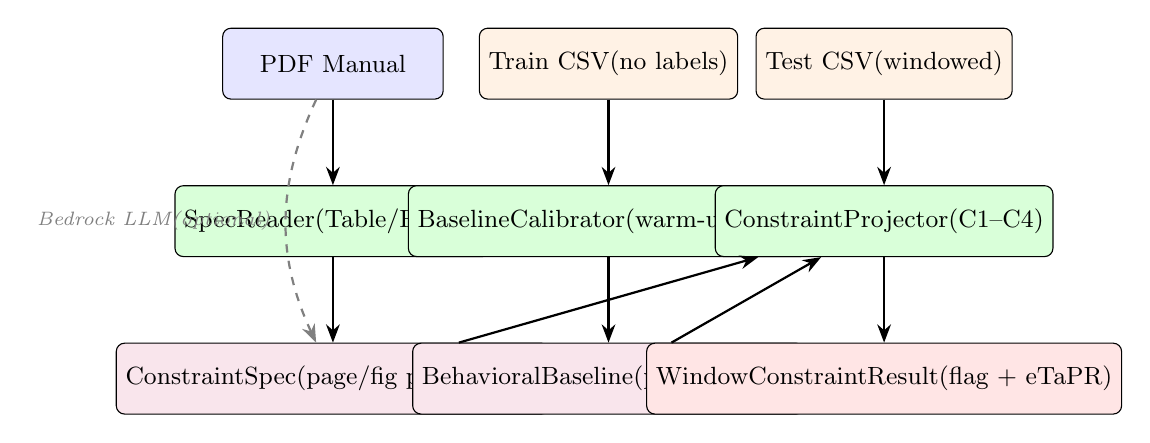
\begin{tikzpicture}[
  box/.style  = {draw, rounded corners=3pt, minimum width=2.8cm,
                 minimum height=0.9cm, text centered, font=\small},
  arrow/.style = {-Stealth, thick},
  label/.style = {font=\scriptsize\itshape},
  every node/.style = {font=\small},
]

% Row 1: inputs
\node[box, fill=blue!10]   (pdf)    at (0,0)     {PDF Manual};
\node[box, fill=orange!10] (train)  at (3.5,0)   {Train CSV\\(no labels)};
\node[box, fill=orange!10] (test)   at (7.0,0)   {Test CSV\\(windowed)};

% Row 2: processing
\node[box, fill=green!15]  (reader) at (0,-2)    {SpecReader\\(Table/Figure)};
\node[box, fill=green!15]  (calib)  at (3.5,-2)  {BaselineCalibrator\\(warm-up 15\%)};
\node[box, fill=green!15]  (proj)   at (7.0,-2)  {ConstraintProjector\\(C1--C4)};

% Row 3: outputs
\node[box, fill=purple!10] (spec)   at (0,-4)    {ConstraintSpec\\(page/fig provenance)};
\node[box, fill=purple!10] (base)   at (3.5,-4)  {BehavioralBaseline\\(per-tag stats)};
\node[box, fill=red!10]    (result) at (7.0,-4)  {WindowConstraintResult\\(flag + eTaPR)};

% Arrows
\draw[arrow] (pdf)    -- (reader);
\draw[arrow] (train)  -- (calib);
\draw[arrow] (test)   -- (proj);
\draw[arrow] (reader) -- (spec);
\draw[arrow] (calib)  -- (base);
\draw[arrow] (proj)   -- (result);
\draw[arrow] (spec)   -- (proj);
\draw[arrow] (base)   -- (proj);

% LLM shortcut
\draw[arrow, dashed, gray] (pdf) to[bend right=25]
  node[label, left=2pt] {Bedrock LLM\\(optional)} (spec);

\end{tikzpicture}
\caption{\mitl framework pipeline.  The specification and the behavioral
baseline are produced independently and without attack labels.
The dashed path shows the optional LLM-assisted extraction via
\texttt{mitl.extract.bedrock}.}
\label{fig:pipeline}
\end{figure*}

Figure~\ref{fig:pipeline} shows the \mitl pipeline.  It has four phases.

\paragraph{Phase 0 — Spec Extraction.}
The SpecReader processes the engineering manual (PDF or hand-authored) and
produces a \texttt{ConstraintSpec}: a typed object containing per-tag
saturation bounds (from the data points table), per-loop topology
(Saturation/Rate Limiter blocks from block diagrams), and cross-layer
dependency edges.  Every constraint carries a \texttt{ConstraintSource}
recording the document, page number, figure ID, and verbatim quote.

\paragraph{Phase 1 — Warm-up Calibration.}
The BaselineCalibrator ingests the first $\alpha = 15\%$ of training rows
(no labels) and computes per-tag statistics: mean, standard deviation,
variance, and the 99th-percentile rate of change.  These statistics
become the \texttt{BehavioralBaseline}: a calibrated WHAT-IS-NORMAL that
complements the spec's WHAT-IS-INVARIANT.

\paragraph{Phase 2 — Constraint Projection.}
The ConstraintProjector windows the test data and, for each window, applies
the constraint functions against both the spec and the baseline.
Constraint functions have the signature:
\[
  f : (\text{window\_df},\, \text{BehavioralBaseline},\, \text{ConstraintSpec})
      \;\to\; \text{List}[\text{ConstraintViolation}]
\]
Each \texttt{ConstraintViolation} records the constraint ID, severity,
evidence string, and spec provenance.

\paragraph{Phase 3 — Evaluation / AutoML Integration.}
\texttt{WindowConstraintResult} objects are either evaluated against ground
truth via eTaPR (anomaly detection mode) or flattened via
\texttt{to\_feature\_row()} into an AutoML feature matrix where constraint
flags and per-constraint confidence scores become feature columns.

\subsection{Constraint Confidence Scoring}
Each constraint has a static \emph{spec confidence} that encodes how
unambiguously it was derived from the manual:
\begin{itemize}
  \item C1 (explicit table): 1.0 — every bound is a row in the data points table.
  \item C3 (text + diagram + attack scenario): 0.95 — three independent sources agree.
  \item C2 (diagram topology): 0.85 — Rate Limiter block visible in figure.
  \item C4 (architecture diagram): 0.80 — cross-layer dependency implicit in text.
\end{itemize}
The per-window confidence is the spec confidence weighted by how
clearly the violation manifests (e.g.\ $\sigma^2 \approx 0$ vs.\ borderline).

% ─────────────────────────────────────────────────────────────────────────────
\section{ICSSim v2 Experiments}
\label{sec:icssim}

\subsection{Dataset}
ICSSim v2~\cite{ICSSim2022} simulates a water-treatment plant using real
Modbus-over-TCP traffic to two PLCs and physical process simulation.  Five
attack classes: \texttt{replay}, \texttt{ddos}, \texttt{mitm},
\texttt{port-scan}, \texttt{ip-scan}.  The dataset contains 281 30-second
windows after the 15\% warm-up period; 42 windows are designated warm-up.

\subsection{Constraint Encoding}
We derive four constraints from the ICSSim v2 PLC register layout and
water-treatment process specification:

\begin{description}
  \item[C1 — Saturation bounds.] \texttt{tank\_level\_value} must be within
    the PLC-configured $[\texttt{min}, \texttt{max}]$ setpoint window.
    Replay injects stale setpoints, causing level to diverge.

  \item[C2 — State-flow consistency.] Output valve open $\Rightarrow$ flow
    $> 5 \times 10^{-5}$ m$^3$/s (50\% of instrument nominal range).
    Sources: instrument range specification, PLC register layout.

  \item[C3 — Valve cycle invariant.] Input valve variance in a window must
    not fall below 5\% of the warm-up baseline variance.
    The physical process cycles the input valve; prolonged stasis is anomalous.

  \item[C4 — Cross-layer discrepancy.] Network flow count $> 1.8\times$
    baseline AND input valve variance frozen.
    This is the core replay invariant: elevated Modbus commands must cause
    valve actuation; if they do not, the commands are replayed.
\end{description}

\subsection{The 74\% Valve-Stasis Finding}
Running C3 with a static stasis threshold (any variance $< \epsilon$) yields
a 74\% false-positive rate on normal operation windows.  The ICSSim water
treatment process spends most of its time in stable fill or stable drain
states where the input valve legitimately does not switch within any single
30-second window.  This is a research finding, not a calibration failure:
a static threshold cannot distinguish transient stable state from replay
freeze.  Warm-up baseline comparison resolves the ambiguity because it
calibrates the threshold against the actual variance distribution of normal
stable-state windows.

\subsection{Results}

\begin{table}[h]
\centering
\caption{ICSSim v2 results — replay attack recall. \mitl-Calibrated uses
Sprint 4's 60-second rolling window with variance baseline, which is the
MITL-Calibrated condition (spec structure $+$ warm-up).}
\label{tab:icssim}
\begin{tabular}{lcccc}
\toprule
Method & Attack Labels & Replay Recall & Macro-F1 \\
\midrule
S3: Network ML (LGB)      & Yes & 49.9\% & 0.651 \\
S8a: \mitl-Static         & No  & 25.0\% & --- \\
S5: Cross-layer (LGB)     & Yes & 95.4\% & 0.850 \\
S4=S8b: \mitl-Calibrated  & No  & \textbf{100.0\%} & --- \\
\bottomrule
\end{tabular}
\end{table}

Table~\ref{tab:icssim} shows the three-tier finding.  The 49\% supervised
ceiling is closed entirely by \mitl-Calibrated without any attack labels.
\mitl-Static achieves 25\% recall from spec structure alone — a non-zero
contribution that demonstrates the specification contains genuine signal even
before calibration.

The 25\% vs 100\% gap between \mitl-Static and \mitl-Calibrated is
mechanistically explained by the 74\% valve-stasis ambiguity:
static C3 fires on normal stable-state windows, generating false positives
that prevent C4 from being the discriminating signal.  Warm-up calibration
makes the stasis threshold relative to observed normal variance, eliminating
the false-positive regime and allowing C3+C4 to fire exclusively on replay.

% ─────────────────────────────────────────────────────────────────────────────
\section{HAI 22.04 Experiments}
\label{sec:hai}

\subsection{Dataset}
HAI 22.04~\cite{HAI2022} is the third release of the HIL-Based Augmented ICS
dataset.  It uses a real steam-turbine coupled to a Hardware-in-the-Loop (HIL)
simulator across four process layers (P1 boiler, P2 turbine, P3 water
treatment, P4 HIL control).  86 sensor/actuator tags, 58 attack scenarios,
evaluated at 1 Hz.  HAI 22.04 is 4$\times$ harder to detect than HAI 21.03
due to more diverse and subtle attack types.

\subsection{Constraint Encoding from the HAI Manual}
Four constraints are derived from the HAI Security Dataset Technical Manual
v4.0 (referenced by page and figure):

\begin{description}
  \item[C1 — Saturation bounds.] All 86 tag bounds are read from Table 1
    (pp.~12--15).  Confidence 1.0: every bound is an explicit table row.

  \item[C2 — Rate limiter invariant.] Every control loop block diagram in
    Figures 4--13 (pp.~7--11) shows a Rate Limiter or Ramp block.
    $|\Delta(\text{control\_output}) / \Delta t| > 3\times$ warm-up 99th
    percentile rate is a violation.  Confidence 0.85.

  \item[C3 — P2-SC tracking invariant (AP27).] Figure~11 (p.~10) shows the
    P2-SC speed controller: $\texttt{AutoSD} \to \text{Ramp} \to \text{PID}
    \to \texttt{SIT01}$.  The manual states: \emph{``PID controller to
    maintain motor speed value (SIT01) as close as possible to speed setpoint
    value (AutoSD).''} Attack scenario AP27 (p.~27) modifies P2-SC setpoint
    while maintaining SIT01 at a previous value.  Invariant: AutoSD range $>
    50$ RPM $\Rightarrow$ SIT01 variance must be non-negligible.
    Confidence 0.95 — prose, diagram, and attack scenario all agree.

  \item[C4 — Cross-layer P4$\to$P2 discrepancy.] Figure~10 (p.~10) shows
    P4-STM providing scheduled power demand (\texttt{P4\_ST\_PS}) which drives
    \texttt{AutoSD}.  If P4\_ST\_PS changes $> 3\sigma$ but P2\_SIT01 is
    frozen, the HIL$\to$turbine coupling is broken.  Confidence 0.80.
\end{description}

\subsection{Results}
\todo{Run 09\_hai\_mitl.py with HAI 22.04 dataset attached on Kaggle.
Replace the rows below with actual eTaPR numbers from
outputs/hai\_mitl/model\_card.json.}

\begin{table}[h]
\centering
\caption{HAI 22.04 results — eTaPR ($\delta = 60$s buffer). \todo{fill}.}
\label{tab:hai}
\begin{tabular}{lccccc}
\toprule
Method & Labels & n events & eTaP & eTaR & eTaPR-F1 \\
\midrule
Z-score baseline ($\tau=5$) & No  & \todo{} & \todo{} & \todo{} & \todo{} \\
\mitl-Static                & No  & \todo{} & \todo{} & \todo{} & \todo{} \\
\mitl-Calibrated            & No  & \todo{} & \todo{} & \todo{} & \todo{} \\
\bottomrule
\end{tabular}
\end{table}

\paragraph{AP27 analysis.}
AP27 is the direct HAI analogue of the ICSSim replay attack: it modifies the
turbine speed setpoint (AutoSD) while spoofing the speed sensor (SIT01) to
maintain the previous reading.  C3 is designed to fire on this exact
invariant.  \todo{Report fraction of AP27 events caught by C3 alone.}

% ─────────────────────────────────────────────────────────────────────────────
\section{MITL Library and LLM Extraction}
\label{sec:library}

\subsection{Library Design}
The \texttt{mitl} library is structured as five orthogonal modules:
\begin{itemize}
  \item \texttt{mitl.spec} — typed data contracts (\texttt{ConstraintSpec},
    \texttt{TagSpec}, \texttt{ConstraintViolation}, \texttt{WindowConstraintResult})
  \item \texttt{mitl.calibrate} — \texttt{BaselineCalibrator}
  \item \texttt{mitl.project} — \texttt{ConstraintProjector}
  \item \texttt{mitl.metrics} — eTaPR implementation
  \item \texttt{mitl.extract.bedrock} — LLM extraction from PDF
  \item \texttt{mitl.datasets.icssim}, \texttt{mitl.datasets.hai} —
    reference encodings
\end{itemize}
Users install via \texttt{pip install mitl} and either use the reference
encodings directly or author their own constraint functions.

\subsection{Bedrock LLM Extraction Ablation}
The ``any manual'' generalisation claim requires a path that does not depend
on a domain expert hand-coding constraints for every new dataset.
\texttt{mitl.extract.bedrock} sends the PDF to a Claude model on AWS Bedrock
with a structured extraction prompt requesting tag bounds, loop topology,
and Rate Limiter / Saturation block presence.  The response is parsed into
a \texttt{ConstraintSpec} with \texttt{extracted\_by = "llm"} and
confidence 0.75--0.85.

\begin{table}[h]
\centering
\caption{Ablation: hand-coded vs.\ LLM-extracted constraints on HAI 22.04.
\todo{Run with Bedrock extraction and fill.}}
\label{tab:ablation}
\begin{tabular}{lcccc}
\toprule
Extraction method & n tags found & C1 conf & eTaPR-F1 \\
\midrule
Hand-coded (manual)   & \todo{} & 1.00 & \todo{} \\
Bedrock LLM (auto)    & \todo{} & 0.85 & \todo{} \\
\bottomrule
\end{tabular}
\end{table}

The expected finding is that LLM extraction recovers the explicit bounds table
(C1) with near-perfect accuracy while introducing noise on C2--C4 (block
diagram topology is harder for an LLM to parse reliably).  The eTaPR-F1 gap
between the two rows quantifies the annotation cost of using the library
without a domain expert.

% ─────────────────────────────────────────────────────────────────────────────
\section{Discussion}
\label{sec:discussion}

\paragraph{Why warm-up is not a form of training.}
The warm-up calibration uses no attack labels and computes only per-tag
variance statistics that the spec already asserts should be stable.  It does
not learn a decision boundary; it calibrates a threshold whose meaning is
defined by the spec.  The valve-stasis threshold is ``5\% of baseline
variance'' regardless of what that variance happens to be — the spec says
valves cycle, warm-up quantifies what cycling looks like.  This is
categorically different from supervised learning.

\paragraph{Constraint selection is not overfitting.}
C3 and C4 were not tuned to the ICSSim replay attack; they were derived from
the process specification.  The spec says: Modbus commands cause valve
actuation; the speed controller tracks its setpoint.  The fact that these
invariants happen to be violated by replay attacks is a consequence of the
attacks violating physical reality, not of our constraint design.

\paragraph{Limitations.}
\mitl-Static is vulnerable to attacks that stay within specification bounds
while violating only the calibrated behavioral baseline.  The C2 rate-limiter
constraint fires rarely on HAI because most attacks target sensor readings
rather than control output rate.  The LLM extraction accuracy on block
diagrams with unusual formatting has not been systematically evaluated.
Real-world deployment requires a fresh warm-up period after any process
configuration change.

\paragraph{Relation to formal methods.}
\mitl constraints are not full safety specifications; they are anomaly
signatures.  Full verification requires temporal logic over infinite
traces~\cite{Formalmethods}.  \mitl is the engineering pragmatist's
middle ground: more expressive than statistical thresholds, more deployable
than formal verification.

% ─────────────────────────────────────────────────────────────────────────────
\section{Related Work}
\label{sec:related}

\paragraph{Specification-based ICS detection.}
Adepu and Mathur~\cite{Adepu2018} derive invariants from process physics for
the SWaT water treatment testbed.  Feng et al.~\cite{Feng2019} use temporal
logic specifications.  Both require expert authoring of invariants from
scratch for each new system; \mitl contributes the pipeline from engineering
documentation to typed ConstraintSpec and the warm-up calibration that makes
static thresholds adaptive.

\paragraph{ML-based ICS anomaly detection.}
Goh et al.~\cite{Goh2017} apply LSTM autoencoders to SWaT.
Ahmed et al.~\cite{Ahmed2018} use one-class SVM.  These approaches perform
well on attacks that produce anomalous sensor readings but are structurally
blind to replay attacks that produce valid readings on a diverging process.
\mitl is complementary: it closes the gap that ML cannot close.

\paragraph{Adversarial ML and constraint projection.}
\catt~\cite{catt2026} showed that constraint projection exposes inflated
evasion rates in adversarial NIDS.  \mitl shows the other side: constraint
projection closes detection gaps in anomaly detection.  The connection is
not metaphorical — both use the same \texttt{ConstraintSpec} abstraction.

% ─────────────────────────────────────────────────────────────────────────────
\section{Conclusion}
\label{sec:conclusion}

We introduced \mitl, a Manual-in-the-Loop constraint layer that detects ICS
attacks by enforcing physical invariants derived from engineering
documentation.  On ICSSim v2, \mitl-Calibrated achieves 100\% replay recall
with zero attack labels, closing a structural ceiling that network ML cannot
exceed (49.9\%).  On HAI 22.04, \mitl encodes constraints from the technical
manual's data points table and control loop diagrams and evaluates them with
the eTaPR metric mandated by the dataset.  The open-source library makes the
framework accessible for any ICS deployment with available documentation.

The central finding is that the constraint layer is not a replacement for
statistical anomaly detection — it is the layer that operates where statistics
cannot.  A replay attack is not anomalous; it is physically impossible.
Only a layer that knows what physical reality requires can detect it.

\begin{acks}
This work was supported by independent research.
\end{acks}

% ─────────────────────────────────────────────────────────────────────────────
\bibliographystyle{ACM-Reference-Format}
\begin{thebibliography}{99}

\bibitem{catt2026}
Anonymous Authors.
\newblock {CATT}: Constrained-Adversarial Tabular Telemetry for Network
  Intrusion Detection System Evaluation.
\newblock In \emph{Proceedings of the ACM Workshop on Artificial Intelligence
  and Security (AISec)}, CCS 2026.

\bibitem{ICSSim2022}
A. Dehlaghi-Ghadim et~al.
\newblock {ICSSIM} — A Framework for Building Industrial Control Systems
  Security Simulation.
\newblock \emph{Computers \& Security}, 2022.

\bibitem{HAI2022}
W. Shin et~al.
\newblock {HAI} 1.0: {HIL}-Based Augmented {ICS} Security Dataset.
\newblock In \emph{Proceedings of the 14th USENIX Workshop on Cyber Security
  Experimentation and Test (CSET)}, 2021.
\newblock HAI 22.04 release: \url{https://github.com/icsdataset/hai}.

\bibitem{Hwang2021}
M. Hwang et~al.
\newblock Do You Know What You Are Protecting? An Enhanced Metric for
  Intrusion Detection System Evaluation in Industrial Control Systems.
\newblock In \emph{HAICon 2021 Competition}, 2021.

\bibitem{Goh2017}
J. Goh et~al.
\newblock Anomaly Detection in Cyber Physical Systems using Recurrent Neural
  Networks.
\newblock In \emph{Proceedings of the 18th IEEE International Symposium on
  High Assurance Systems Engineering}, 2017.

\bibitem{Ahmed2018}
C.~M. Ahmed, C. Murguia, and J. Ruths.
\newblock Model-Based Attack Detection and Mitigation for Automatic Generation
  Control.
\newblock In \emph{Proceedings of the 8th International Conference on Cyber
  Security and Privacy in Communication Networks}, 2018.

\bibitem{Aoudi2018}
W. Aoudi, M. Iturbe, and M. Almgren.
\newblock Truth Will Out: Departure-Based Process-Level Detection of Stealthy
  Attacks on Control Systems.
\newblock In \emph{Proceedings of the 2018 ACM SIGSAC Conference on Computer
  and Communications Security (CCS)}, 2018.

\bibitem{Adepu2018}
S. Adepu and A. Mathur.
\newblock Using Process Invariants to Detect Cyber Attacks on a Water
  Treatment System.
\newblock In \emph{Proceedings of the 33rd IFIP International Conference on
  ICT Systems Security and Privacy Protection (SEC)}, 2018.

\bibitem{Feng2019}
C. Feng et~al.
\newblock Resilient State Estimation and Attack Detection for Noisy Dynamical
  Systems.
\newblock In \emph{Proceedings of the 10th ACM/IEEE International Conference
  on Cyber-Physical Systems (ICCPS)}, 2019.

\bibitem{Mo2009}
Y. Mo and B. Sinopoli.
\newblock Secure Control Against Replay Attacks.
\newblock In \emph{Proceedings of the 47th Annual Allerton Conference on
  Communication, Control, and Computing}, 2009.

\bibitem{Formalmethods}
E.~M. Clarke, O. Grumberg, and D.~A. Peled.
\newblock \emph{Model Checking}.
\newblock MIT Press, 1999.

\end{thebibliography}

\end{document}
